%%
%
% Body
%
%%
\section{WRAMP Stack Frame}

A stack is a term used to describe a `first in, last out' buffer. New
items are placed on the top of the stack, and must be removed before
older items. Two terms are commonly used to refer to the operations of
adding to, and removing values from a stack. A push operation puts a
new value at the very top of the stack, and a pop operation removes the
item from the top of the stack. These are the only operations allowed to
be performed on a stack, and there is no way to remove an older item
before a newer one. Stacks provide an ideal mechanism for passing
parameters to a function and providing storage for local variables and
temporary results inside a function. This document describes the
reasons a stack is used on the WRAMP architecture, how the stack is
created, and the conventions surrounding its use.

The WRAMP processor itself does not directly support a stack, but
it is possible to setup a stack in software. To achieve this, a block
of memory for the stack to reside in must be set aside. On the Basys
board, \WRAMPmon\ does this for you. The stack starts at the top of
memory, with new items placed at lower memory addresses. Because of
this, stacks on the WRAMP architecture are often referred to as
growing downwards.

%%%
%
% PUSH FIGURE
%
%%%
\begin{figure}[!hb]
\begin{center}
\begin{footnotesize}
\begin{tabular}{|c|c|c|}

\hline
%% Text....
\begin{minipage}[l]{7cm}
\vspace{\topsep}
\begin{verbatim}

push:
      # move the stack pointer down
      # by one to create space for 
      # a value to be pushed onto 
      # the stack.

      subui $sp, $sp, 1

      # store the contents of $2 onto
      # the new space on the stack

      sw $2, 0($sp)

\end{verbatim}
\end{minipage}
&
%% Fig before
\begin{minipage}[c]{3.5cm}
\begin{center}
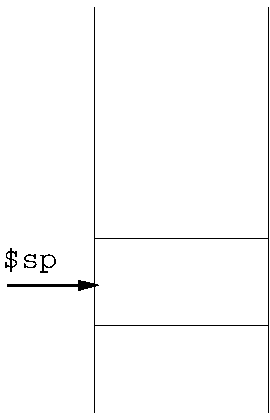
\includegraphics[width=2.2cm]{stack_fig1_a.eps}
%\vspace{0.1cm}

\emph{before}\\
\end{center}
\end{minipage}

&
%% Fig after
\begin{minipage}[c]{3.5cm}
\begin{center}
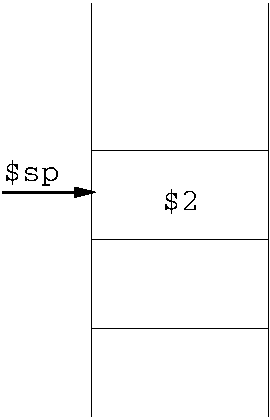
\includegraphics[width=2.2cm]{stack_fig1_b.eps}


\emph{after}\\
\end{center}
\end{minipage}
\\
\hline
\end{tabular}
\begin{center}
\small{
\textbf{(a) WRAMP code}
\hspace{3.5cm}
\textbf{(b) Stack Diagrams}
}
\end{center}

\caption{Push}
\label{fig:stack_push}
\end{footnotesize}
\end{center}
\end{figure}
%%%
%
% End of PUSH figure
%
%%%

To place new items onto and remove existing items from the stack you
need a way to know the current address of the top of the stack. To
allow this, a register is set aside to store this address. This
register is referred to as the ``top of stack'' pointer, or more often
just the ``stack pointer''. By WRAMP convention, the stack pointer is stored
in register 14 and is referred to as \src{\$sp} in WRAMP assembly code.
Figure \ref{fig:stack_push}(a) shows example WRAMP code to ``push'' a new
value onto the stack and (b) shows the stack before and after the push operation. Figure \ref{fig:stack_pop} shows the WRAMP code and stack diagrams for a pop
operation.

%%%
%
% POP FIGURE
%
%%%
\begin{figure}[!ht]
\begin{center}
\begin{footnotesize}
\begin{tabular}{|c|c|c|}

\hline
%% Text....
\begin{minipage}[l]{7cm}
\vspace{\topsep}
\begin{verbatim}

pop:
      # pop into register 3 the value
      # stored on the top of the
      # stack

      lw $3, 0($sp)

      # Move the stack pointer up
      # by one to remove item

      addui $sp, $sp, 1

\end{verbatim}
\end{minipage}
&
%% Fig before
\begin{minipage}[c]{3.5cm}
\begin{center}
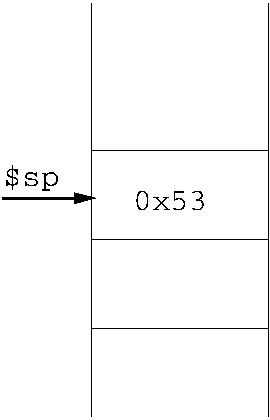
\includegraphics[width=2.2cm]{stack_fig2_a.eps}
%\vspace{0.3cm}

\emph{before}\\
\end{center}
\end{minipage}

&
%% Fig after
\begin{minipage}[c]{3.5cm}
\begin{center}
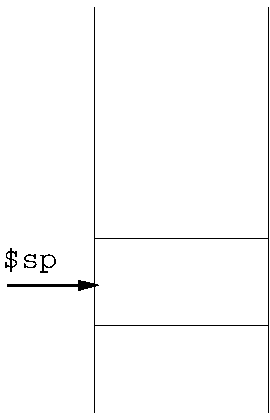
\includegraphics[width=2.2cm]{stack_fig2_b.eps}

%\vspace{0.3cm}
\emph{after}\\
\end{center}
\end{minipage}
\\
\hline
\end{tabular}
\begin{center}
\small{
\textbf{(a) WRAMP code}
\hspace{3.5cm}
\textbf{(b) Stack Diagrams}
}
\end{center}

\caption{Pop}
\label{fig:stack_pop}
\end{footnotesize}
\end{center}
\end{figure}
%%%
%
% End of POP figure
%
%%%
\vspace{0.2cm} %Push to the next page

\section{WRAMP Stack Conventions}
On the WRAMP architecture the stack is used to:

\begin{itemize}
\item store local variables that are not stored in registers
\item temporarily store the contents of registers so that a subroutine can use them while making sure the previous contents are preserved.
\item pass parameters to a subroutine
\end{itemize}

%%%
%
% Figure 3
%
%%%
\begin{figure}[!hbt]
\begin{footnotesize}
\begin{center}
\begin{tabular}{|p{10cm}|}
\hline
\begin{verbatim}
parent:
       addi $3, $0, 5
loop:
       beqz $3, endloop
        ...
       jal child
        ...
       subi $3, $3, 1
       j loop

endloop:
       j exit

child:
        ...
       add $3, $4, $5
        ...
       jr $ra
\end{verbatim}
\\
\hline
\end{tabular}
\end{center}
\end{footnotesize}
\caption{Incorrect Function} 
\label{fig:problemcode}
\end{figure}

\section{Saving Registers}
When a program contains a number of subroutines that can call each
other, a set of conventions is required to ensure that a subroutine
does not use a register and modify values that a parent subroutine is
also using. For example consider the code sequence in Figure
\ref{fig:problemcode}. Notice that the section of code labelled
\src{parent} is using \src{\$3} as a loop counter that decrements each
time through the loop. Inside this loop is a call to the subroutine
\src{child} that uses \src{\$3} to store an intermediate result. This
would overwrite the loop counter value stored in that register by the
subroutine \src{parent}. While it would be possible in this simple
sequence to rearrange the code to fix the problem, it will not always
be possible to do so. To ensure problems like this do not occur in
code there needs to be a set of conventions controlling the way
registers are used.

The convention used in the WRAMP architecture is that all subroutines
must save the contents of a register to the stack before it can use
it. The value must then be restored from the stack before the
subroutine exits. It should be noted that it is up to the programmer
to ensure these conventions are followed and the processor does not
enforce them in any way. For code generated by a C compiler, the
compiler must ensure that these same conventions are followed. Figure
\ref{fig:correctcode} shows the corrected program that follows the
conventions.

When a subroutine is called using the \src{jal} instruction, the
return address for the subroutine is placed in register 15
(\src{\$ra}). If this subroutine then uses \src{jal} to call another
subroutine it will overwrite its own return address. Because of this,
any subroutine that is going to call another subroutine needs to save
\src{\$ra} onto the stack before calling the routine and restore it
before it returns. Figure \ref{savera} gives an example of this.


%%
%
% Figure 4
%
%%%
\begin{figure}[!hb]
\begin{footnotesize}
\begin{center}
\begin{tabular}{|p{10cm}|}
\hline
\begin{verbatim}
parent:
       addi  $3, $0, 5
loop:
       beqz  $3, endloop
        ...
       jal   child
        ...
       subi  $3, $3, 1
       j     loop

endloop:
       j exit

child:
        ...
       # save register 3 before we overwrite
       # the contents of it
       subui $sp, $sp, 1
       sw    $3, 0($sp)

       add   $3, $4, $5
        ...
       # restore the old contents of register
       # 3 before we return
       lw    $3, 0($sp)
       addui $sp, $sp, 1

       jr    $ra
\end{verbatim}
\\
\hline
\end{tabular}
\end{center}
\end{footnotesize}
\caption{Correct Function}
\label{fig:correctcode}
\end{figure}

There is one exception to the rule that all registers must be
saved. For reasons discussed in the next section, register 1
(\src{\$1}) never needs to be saved or restored.

\section{Parameter Passing}
In Chapter \ref{chapter:intro}, parameters were passed to
subroutines using regsiters. While this works in this simple case
consider what would happen if a subroutine required a large number of
parameters or called other subroutines. It is not difficult to see that
with a large program it would not take long to exhaust the registers
available to the programmer on the WRAMP processor.

%%%
%
% Figure 5
%
%%%
\begin{figure}[!htbp]
\begin{footnotesize}
\begin{center}
\begin{tabular}{|p{10cm}|}
\hline
\begin{verbatim}
child:
       # save the return address before we
       # call our subroutine
       subui $sp, $sp, 1
       sw $ra, 0($sp)

       jal my_child
        ...

       # get our return address back off of the
       # stack so we can return there.
       lw $ra, 0($sp)
       addui $sp, $sp, 1

       jr $ra
\end{verbatim}
\\
\hline
\end{tabular}
\end{center}
\end{footnotesize}
\caption{Calling a Function}
\label{savera}
\end{figure}

A convention needs to be defined so that a subroutine knows how to
find the parameters it has been passed, and knows how to pass
parameters to subroutines it calls.

On the WRAMP processor the convention is to pass all parameters to a
subroutine using the stack. Before a subroutine is called all of the
parameters that are going to be passed to it must first be pushed onto
the stack. Parameters appear on the very top of the stack when a
subroutine is entered. If code is being generated for a C function
call, then the convention is to push the parameters onto the stack in
the reverse order so that the first C parameter ends up on the top of
the stack just before the function is called. Figure
\ref{fig:parampassing}(a) shows a C function call, (b) WRAMP code to
implement it and (c) a diagram of the stack at the time of the
function call.

%%%
%
% Fig6: Param Passing
%
%%%
\begin{figure}[!hbtp]
\begin{center}
\begin{footnotesize}
\begin{tabular}{|c|c|c|}
\hline
\begin{minipage}[t]{4.8cm}
\begin{verbatim}

cat(first, second, third);

\end{verbatim}
%$
\end{minipage}
&
\begin{minipage}[c]{5.5cm}
\vspace{\topsep}
\begin{verbatim}

# push the third parameter on
subui $sp, $sp, 1
sw $3, 0($sp)

# push the second parameter on
subui $sp, $sp, 1
sw $4, 0($sp)

# push the first parameter on
subui $sp, $sp, 1
sw $5, 0($sp)

jal cat

# remove all three parameters
addui $sp, $sp, 3

\end{verbatim}
%$
\end{minipage}
&
\begin{minipage}{4.2cm}
\begin{center}
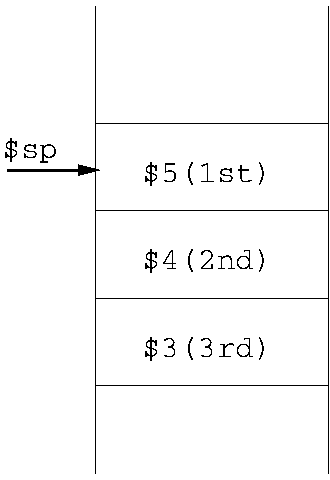
\includegraphics[width=3cm]{stack_fig6_a.eps}
\end{center}
\end{minipage}\\
\hline
\end{tabular}
\\
\textbf{(a) C code}
\hspace{3cm}
\textbf{(b) WRAMP code}
\hspace{3cm}
\textbf{(c) Stack before call}\\

\caption{Passing Parameters to a Function}
\label{fig:parampassing}
\end{footnotesize}
\end{center}
\end{figure}

As you will notice in the previous example, a significant proportion of
the WRAMP code is associated with manipulating the stack pointer. An
alternative and more efficient approach is to calculate the maximum
size that a stack will grow to in a function and pre-allocate this
space as the function is entered. Just before this "parent" function
calls another function it copies the parameters to the appropriate
place in the pre-allocated space. If the function accepts one
parameter, that parameter must be placed at the top of the stack. If a
function accepts two parameters the first parameter must be placed at
the top of the stack and the second placed beneath it. If you think
of the parameters as a list numbered from zero, the position of any
parameter can be calculated as follows:

\begin{center}
$Address = \$sp + ParameterNumber$\\
\end{center}

For example if a function \src{cat(first, second, third)} is going to
be called then first will be placed at \mbox{\src{\$sp} + 0}, second
at \mbox{\src{\$sp} + 1} and third at \mbox{\src{\$sp} + 2}. Figure
\ref{fig:paramcalling}(a) shows an example C code sequence containing two
function calls (one with a single parameter and one with three
parameters) and Figure \ref{fig:paramcalling}(b) shows the WRAMP
assembly code for this sequence.

Once a subroutine has been called it then has to retrieve these
parameters off of the stack so that it can use them. This requires a
number of loads from the current stack. The important part to notice
is that these are not pop operations, as they do not reduce the size
of the stack. The function is simply looking into the stack of the
function that called it to discover the parameters it has been called
with. A function must \textbf{\emph{never}} return with the stack
pointer pointing to a different location than when the function was
called.

A function also needs to be able to return a value to its
parent. Traditional languages only ever allow a function to return a
single value, therefore the use of the stack to return a value is
probably over complex. On the WRAMP architecture, values are returned
to the parent in register 1 (\src{\$1}). Because of this fact,
\src{\$1} is the only exception to the rule that all registers must be
returned with their original contents when a function returns. A
function is actually allowed to change the contents of \src{\$1} even
if it doesn't return any value to its parent. Figure
\ref{fig:paramexample} shows a simple maximum function that is passed
two parameters and returns the larger of the two. As this function is
a leaf function (i.e. calls no other functions) it need not save the
contents of its return address.

%%%%
%
% Figure 7
%
%%%%
\begin{figure}[!hbtp]
\begin{footnotesize}
\begin{center}
\begin{tabular}{|c|c|}
\hline
\begin{minipage}[t]{5cm}
\vspace{\topsep}
\begin{verbatim}

 ...
dog(last);
 ...
cat(first, second, third);
 ...

\end{verbatim}
\end{minipage}
&
\begin{minipage}[t]{8cm}
\vspace{\topsep}
\begin{verbatim}

 # allocate the amount of space on the stack
 # to allow for the call with the largest number
 # or parameters. (in this case 3)
 subui $sp, $sp, 3
  ...

 # The parameter 'last' must be placed on the stack
 # and is currently being stored in $6.
 sw $6, 0($sp)

 # Call the function
 jal dog
  ...

 # Put the parameters for cat onto the stack
 sw $5, 0($sp)    # 'first'
 sw $4, 1($sp)    # 'second'
 sw $3, 2($sp)    # 'third'

 # Call the function
 jal cat
  ...

 # remove the space from the stack.
 addui $sp, $sp, 3

\end{verbatim}
\end{minipage}
\\
\hline
\end{tabular}
\\
\textbf{(a) C code}
\hspace{3.5cm}
\textbf{(b) WRAMP code}
\end{center}
\end{footnotesize}

\caption{Calling multiple functions}
\label{fig:paramcalling}
\end{figure}

\section{Local Variables}
So far we have kept all local variables, such as temporary storage,
loop counters etc. in registers. As there are a small number of
registers it would be a major limit to a language to enforce that it
could have no more local variables than the architecture has
registers. To overcome this limit, the stack is set up so that local
variables can be stored on the stack and only be loaded into registers
temporarily as required. A code segment is shown in Figure
\ref{var_example}(a). Figure \ref{var_example}(b) provides an example
of how the WRAMP code would look if the local variables are kept on the
stack. As you can see, even in this small piece of code there is a
large proportion of the code dealing with fetching and storing the
variables to and from the stack. If you are writing C code it is the
job of a compiler to optimise these areas of the assembly code and
reduce to a minimum the number of these load and store instructions.

\section{The Stack Frame}

All of the discussion so far has been treating the uses of the stack as
separate concepts. In reality all of these are used by C functions to create
a concept called the stack frame. The stack frame is an area on the top of the
stack that has a standard format. Inside this block is space for local
variables, register save and parameter passing for the current function. We
precalculate the size of the stack frame by summing the sizes of each of these
areas. We need space for one item on the stack for every local variable, one
item for each register we save, and one item for each parameter of the function
with the largest number of parameters that we call.

For example if we need to setup a stack frame for a function that needs to
store three local variables and save two registers but calls no other function
we will need a stack frame of size 5.

If we have a non-leaf function that needs 3 local variables, save 4 registers
and the return address, and calls two functions, one of which takes 2 parameter
and the other takes 4 parameters, we will need a stack frame of size 12.

The layout for a complete stack frame is shown in Figure \ref{stackframe}

%%%%
%
% Figure 8
%
%%%%
\begin{figure}[!btp]

\begin{center}
\begin{tabular}{|p{10cm}|}
\hline
\begin{scriptsize}
\begin{verbatim}
parent:
       addi $3, $0, 5
loop:
       beqz $3 endloop
        ...
       jal child
        ...
       subi $3, $3, 1
       j loop

endloop:
       j exit

child:
        ...
       # save register 3 before we overwrite
       # the contents of it
       subui $sp, $sp, 1
       sw $3, 0($sp)

       add $3, $4, $5
        ...
       # restore the old contents of register
       # 3 before we return
       lw $3, 0($sp)
       addui $sp, $sp, 1

       jr $ra
\end{verbatim}
\end{scriptsize}
%$
\\
\hline
\end{tabular}
\end{center}
\

\caption{Example}
\label{fig:paramexample}
\end{figure}

%%%%%%%%%%%%%%%%%%%%%%%%%%%%%%%%

\begin{figure}[!hbtp]
\begin{footnotesize}
\begin{center}
\begin{tabular}{|p{8cm}|}
\hline
\\
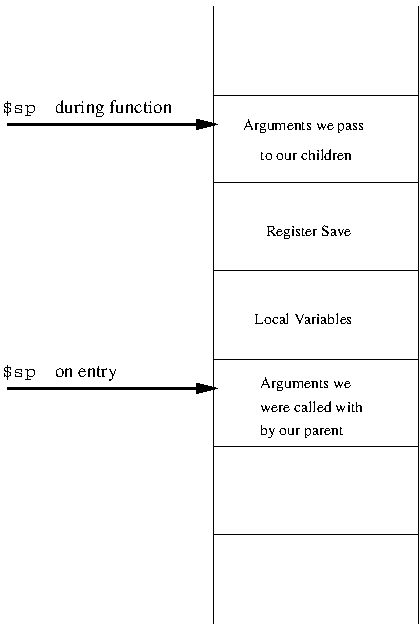
\includegraphics[width=6cm]{stack_fig10.eps}

\\
\hline
\end{tabular}
\end{center}
\end{footnotesize}

\caption{The Stack Frame}
\label{stackframe}
\end{figure}

Figure \ref{stack_example} shows a non-leaf function that calls two
subroutines. The function has zero local variables stored on the
stack, but is a fully compliant function. It sets up a stack frame on
entry and tears it down on exit. It is strongly suggested that you
walk through this code and draw a diagram of the stack frame that this
function creates. Any functions you write that need to be compliant
should contain very similar entry and exit code to this function.

The function is a successive addition multiplication system. It uses a
function called \src{add} to add the two numbers. At the end of the
function it displays the result to the seven segment display using the
\src{writessd} function.

%%%%
%
% Figure 9
%
%%%%
\begin{figure}[!hbtp]
%\begin{footnotesize}
\begin{center}
\begin{tabular}{|c|c|c|}
\hline
\begin{minipage}[t]{5cm}
\begin{scriptsize}
\begin{verbatim}

int i;
int a = 2;
int b = 3;
int result = 0;

for(i = 0; i < a; i++){

   result = result + b;

}

 ...

\end{verbatim}
\end{scriptsize}
\end{minipage}
&
\begin{minipage}[t]{6cm}
\begin{scriptsize}
\begin{verbatim}

func:
       # Allocate space for 4 locals
       subui $sp, $sp, 4

       # Initialise a = 2
       addi $2, $0, 2
       sw $2, 1($sp)

       # Initialise b = 3
       addi $2, $0, 3
       sw $2, 2($sp)

       # Initialise result = 0
       sw $0, 3($sp)

       # Initialise i = 0
       sw $0, 0($sp)

loop:
       # Do the for loop test
       lw $2, 0($sp)  # get i
       lw $3, 1($sp)  # get a
       slt $4, $2, $3
       beqz $4, end

       # perform the loop
       lw $2, 3($sp)  # get result
       lw $3, 2($sp)  # get b
       add $2, $2, $3
       sw $2, 3($sp)  # put result

       # increment i
       lw $2, 0($sp)  # get i
       addi $2, $2, 1
       sw $2, 0($sp)  # put i

       j loop

end:
        ...

\end{verbatim}
\end{scriptsize}
\end{minipage}
&
\begin{minipage}[t]{5cm}
\begin{center}

\vspace{3.5cm}
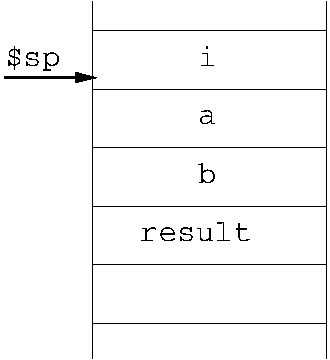
\includegraphics[width=3cm]{stack_fig9_a.eps}

\end{center}
\end{minipage}
\\
\hline
\textbf{(a) C code} & \textbf{(b) WRAMP code} & \textbf{(c) Stack}\\
\hline
\end{tabular}
\end{center}

\caption{Using Variables}
\label{var_example}
\end{figure}

%%%%
%
% Figure 11
%
%%%%
\begin{figure}[!hbtp]
\begin{footnotesize}
\begin{center}
\begin{tabular}{|p{15cm}|}
\hline
\begin{verbatim}

multiply:
        # Setup a stack frame (2 parameters, 5 registers to be saved)
        subui   $sp, $sp, 7
        # Save some registers for us to use
        sw      $6, 2($sp)
        sw      $7, 3($sp)
        sw      $8, 4($sp)
        sw      $9, 5($sp)
        # This is a non-leaf function so we must save the return address
        sw      $ra, 6($sp)

        # Initialise the 'result' variable to zero
        addu    $7, $0, $0
        # Initialise our loop counter
        addu    $6, $0, $0
        # Get our first parameter into $8
        lw      $8, 7($sp)
        # Get our second parameter into $9
        lw      $9, 8($sp)

loop:
        # Use our 1st parameter to control how many times we add our
        # second parameter to itself
        slt     $1, $6, $8
        beqz    $1, exit_loop

        # The first parameter to add is the existing 'result'
        sw      $7, 0($sp)

        # The second parameter we pass is the same as our 2nd parameter
        sw      $9, 1($sp)
        jal     add

        # Save the return value from add back into our 'result' variable
        addu    $7, $0, $1

        # Increment our loop counter
        addui   $6, $6, 1

        j       loop

exit_loop:
        # Write the result to the seven segment display
        sw      $7, 0($sp)
        jal     writessd

        # Return our result to our parent
        addu    $1, $0, $7

        # Restore all the registers we used
        lw      $6, 2($sp)
        lw      $7, 3($sp)
        lw      $8, 4($sp)
        lw      $9, 5($sp)

        # Get our return address back
        lw      $ra, 6($sp)

        # Destroy our stack frame
        addui   $sp, $sp, 7
        # Return
        jr      $ra

\end{verbatim}
%$
\\
\hline
\end{tabular}
\end{center}
\end{footnotesize}

\caption{Example}
\label{stack_example}
\end{figure}
